\documentclass{article}\raggedbottom

% if you need to pass options to natbib, use, e.g.:
% \PassOptionsToPackage{numbers, compress}{natbib}
% before loading nips_2016
%
% to avoid loading the natbib package, add option nonatbib:
% \usepackage[nonatbib]{nips_2016}

%\usepackage{nips_2016}

% to compile a camera-ready version, add the [final] option, e.g.:
% \usepackage[final]{nips_2016}

\usepackage[utf8]{inputenc} % allow utf-8 input
\usepackage[T1]{fontenc}    % use 8-bit T1 fonts
\usepackage[hidelinks]{hyperref}       % hyperlinks
\usepackage{url}            % simple URL typesetting
\usepackage{booktabs}       % professional-quality tables
\usepackage{amsfonts}       % blackboard math symbols
\usepackage{nicefrac}       % compact symbols for 1/2, etc.
\usepackage{cleveref}		
\usepackage{microtype}      % microtypography
\usepackage{listings} %For code in appendix
\lstset
{ %Formatting for code in appendix
	language=Python,
	basicstyle=\footnotesize,
	numbers=left,
	stepnumber=1,
	showstringspaces=false,
	tabsize=1,
	breaklines=true,
	breakatwhitespace=false,
}
\usepackage{mathtools} 
\usepackage{graphicx}
\usepackage{subcaption}
\usepackage{csvsimple}
\usepackage{float}


\title{An Analysis of Image Denoising Techniques}
\usepackage[final]{nips_2016}

% The \author macro works with any number of authors. There are two
% commands used to separate the names and addresses of multiple
% authors: \And and \AND.
%
% Using \And between authors leaves it to LaTeX to determine where to
% break the lines. Using \AND forces a line break at that point. So,
% if LaTeX puts 3 of 4 authors names on the first line, and the last
% on the second line, try using \AND instead of \And before the third
% author name.

\author{
  Benjamin A. Schifman\\
  Department of Electrical and Computer Engineering\\
  University of Arizona\\
  Tucson, AZ 85719 \\
  \texttt{bschifman@email.arizona.edu} \\
  %% examples of more authors
  %% \And
  %% Coauthor \\
  %% Affiliation \\
  %% Address \\
  %% \texttt{email} \\
  %% \AND
  %% Coauthor \\
  %% Affiliation \\
  %% Address \\
  %% \texttt{email} \\
  %% \And
  %% Coauthor \\
  %% Affiliation \\
  %% Address \\
  %% \texttt{email} \\
  %% \And
  %% Coauthor \\
  %% Affiliation \\
  %% Address \\
  %% \texttt{email} \\
}

\begin{document}
 

\maketitle

\begin{abstract}
  Digital denoising techniques are used to filter out unwanted noise in a signal. In images, noisy signals are present in the form of non coherent Salt \& Pepper noise and Gaussian noise to coherent noise introduced inherently from the imager or from signal processing algorithms. This paper examines some of the common methods for removing unwanted noise, along with implementing more adept filtering techniques in the form wavelet filtering. 
\end{abstract}

\section{Introduction}
 This paper explores noise filtering techniques implemented in Python and an available Python image processing library $OpenCV.$ The filters are implemented on images with random Gaussian noise and Salt \& Pepper noise, and their output Peak Signal to Noise Ratios are compared. The two $python$ files are detailed in section \ref{Software_Lisiting}. The standard filters that were implemented using the $OpenCV$ library were the: \textit{blur, gaussian blur, median} and \textit{bilateral} filters and the filter windows were varied in order to generate the optimal resulting filter. The Haar Wavelet Transform was implemented by hand, and the Daubechies 4 wavelet was implemented using the available $PyWavelets$ library after an attempt by hand of the algorithm was unsuccessful.

\section{Methods/Approach}
\subsection{Noise Generation}
Two images were generated with different noise distributions for the purpose of analyzing the efficacy of the different applied filtering techniques. The first noisy image was generated with a normal Gaussian distribution that had been scaled by a factor of $10$. The noise was scaled in order to be more visually evident in the image along with increasing the noise power in the image. Gaussian noise is generally a common form of noise that principally arises in images during acquisition and is caused by a number of factors, a few being poor illumination, high circuitry temperature, and electronic interference. The second noisy image was generated through adding a $0.4\%$ Salt \& Pepper (S\&P) distribution. The S\&P noise added was equally distributed "Salt" white pixels, and "Pepper" black pixels. S\&P noise potentially occurs in images were intermittent and non-reliable image communication systems are present as they can elicit sharp and sudden disturbances in the image signal. The following Figure~\ref{fig:input_images} depicts the original image along with the noise induced images.

\begin{figure}[h!]
	\centering
	\begin{subfigure}[b]{0.45\linewidth}
		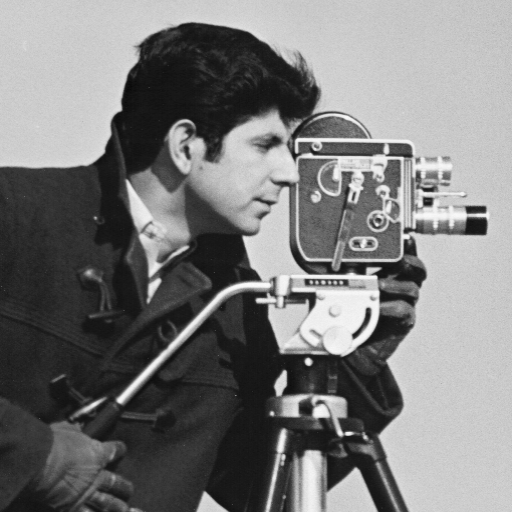
\includegraphics[width=\linewidth]{../../2_Software/data/cman_512_512.png}
		\caption{cman}
	\end{subfigure}
	\begin{subfigure}[b]{0.45\linewidth}
		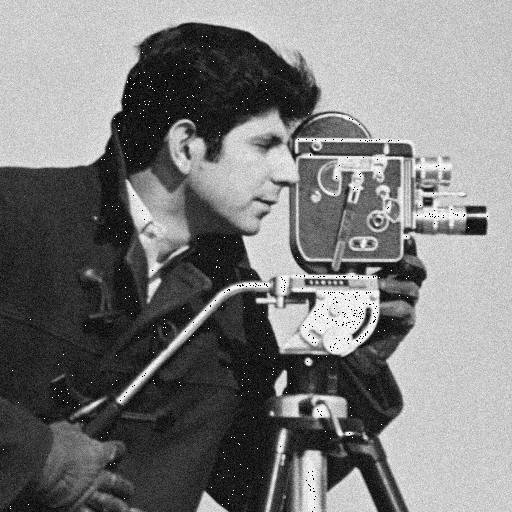
\includegraphics[width=\linewidth]{../../2_Software/data/cman_gnoise.png}
		\caption{cman w\ Gaussian Noise}
	\end{subfigure}
	\begin{subfigure}[b]{0.45\linewidth}
		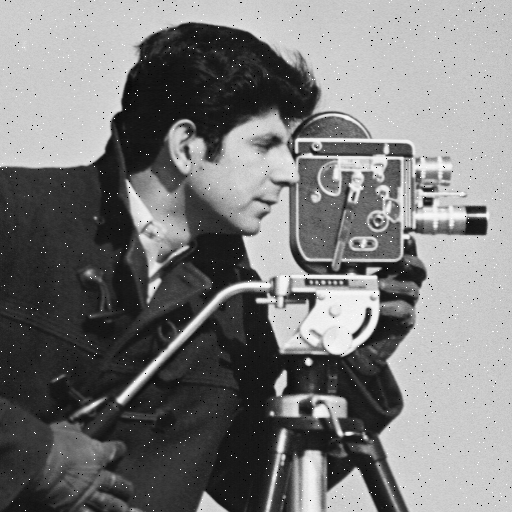
\includegraphics[width=\linewidth]{../../2_Software/data/cman_spnoise.png}
		\caption{cman w\ S\&P Noise}
	\end{subfigure}
	\caption{Input Images}
	\label{fig:input_images}
\end{figure}

\subsection{Peak Signal to Noise Ratio}
In order to analyze the utility of the aforementioned filtering techniques the Peak Signal to Noise Ratios (PSNR) for each filtered image was calculated. The PSNR of an image is the maximum power of an image and the power of the image noise. The following Equation \eqref{eqn:PSNR} details the calculations for PSNR output in decibels (dB) which is the unit that will be continued throughout this paper.
\begin{equation}\label{eqn:PSNR}
PSNR = 10*log_{10}\Big(\frac{MAX^2}{MSE}\Big)
\end{equation}	 
Where $MAX$ is the maximum grayscale pixel value for the image which in this case is an unsigned 8-bit image with a maximum value of 255, and the $MSE$ is the Mean Squared Error between the filtered output image and the noisy image.

\subsection{Standard Filters}
The standard filters described in the following sections were implemented using the available python $OpenCV$ library and can be found in the $standardFilters$ function in the $dataSetup.py$ file. The correct filter lengths were chosen through the process of iterating over odd filter lengths and then observing the corresponding PSNR values from the filters and this can be seen in the following Figure~\ref{fig:filter_length} and in the $dataSetup.py$, $detFilterLength$ funciton. The resultant filter outputs can be found in the the Results section in Figures ~\ref{fig:filter_outputs_1},
~\ref{fig:filter_outputs_2}, ~\ref{fig:filter_outputs_3}, ~\ref{fig:filter_outputs_4}

\begin{figure}[h!]
	\centering
	\begin{subfigure}[b]{0.45\linewidth}
		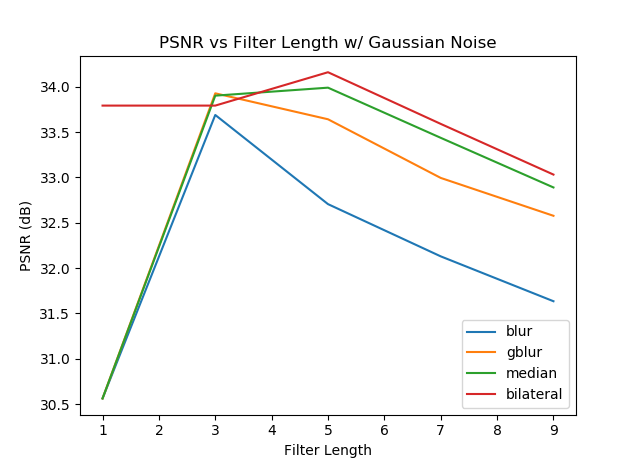
\includegraphics[width=\linewidth]{../../1_Resources/images/filter_length_g.png}
		\caption{Filters w\ Gaussian Noisy Image.}
	\end{subfigure}
	\begin{subfigure}[b]{0.45\linewidth}
		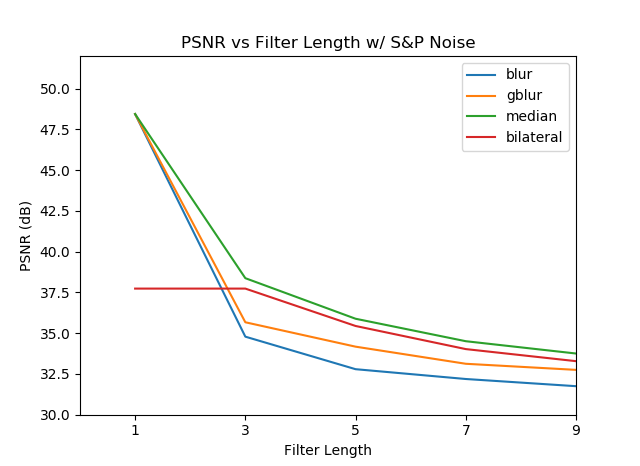
\includegraphics[width=\linewidth]{../../1_Resources/images/filter_length_sp.png}
		\caption{Filters w\ S\&P Noisy Image.}
	\end{subfigure}	
	\caption{PSNR vs. Filter Lengths}
	\label{fig:filter_length}
\end{figure}

\subsubsection{Blur Filtering}
The Blur filter was implemented by convolving the the image with the normalized box window. $OpenCV$, however, implemented all of the convolution process under the hood, so only a specific filter window length was required. In the example of a $3$x$3$ normalized block filter the kernel would look like the following Equation \eqref{eqn:blur}


\begin{equation}\label{eqn:blur}
	K = \frac{1}{9}
	\begin{bmatrix}
	1 & 1 & 1\\
	1 & 1 & 1\\
	1 & 1 & 1
	\end{bmatrix}
\end{equation} 

\subsubsection{Gaussian Blur Filtering}
The Gaussian Blur filter was implemented by convolving the the image with a Gaussian kernel, with the standard deviation of the Gaussian distribution calculated by the length of the filter. In the example of a $3$x$3$ Gaussian  filter the kernel would look like the following Equation \eqref{eqn:gaussian_blur}

\begin{equation}\label{eqn:gaussian_blur}
	K = \frac{1}{16}
	\begin{bmatrix}
	1 & 2 & 1\\
	2 & 4 & 2\\
	1 & 2 & 1
	\end{bmatrix}
\end{equation}

\subsubsection{Median Filtering}
The Median filter was implemented by taking the pixels of the image that were under the kernel filter size and then replacing the central pixel element with the median value.

\subsubsection{Bilateral Fitlering}
The Bilateral Filter is a non-linear, edge preserving filter, and noise reducing smoothing filter. It replaces the intensity of the central pixel value with a weighted average of the other pixels in the filter window


 
\subsection{Haar Wavelet Transform}
The Haar Wavelet Transform (HWT), proposed by the Hungarian mathematician Alfr\'ed Haar is a computationally efficient method for analyzing the local aspects of an image. A key advantage to the use and implementation of the HWT is in it simplicity to compute, along with it being easier to understand than most other wavelet transforms. A great benefit to using the HWT is that it is effective in signal and image compression and the algorithm is memory efficient in that all of the calculations can be done in place, however, the software depicted below uses temporary vectors for ease of following along. The motivation behind the use of the HWT and wavelet transforms in general is that wavelets are a means of expressing a function in a certain basis, but in contrast to Fourier analysis, where the basis is fixed, wavelets provide a general framework with varying orthogonal bases. This is beneficial due to the fact that in Fourier Analysis, and specifically the Discrete Fourier Transform (DFT), the DFT is limited to a fixed frequency content over time in representation of a trigonometric function, and in an image their is often contrast in image data where the characteristics can be vastly different in varying parts of the image. This can provide differenet resolution at different parts of the time-frequency plane \cite{porwik2004haar}. The HWT can be expressed in terms of matrix operations such that the Forward HWT is expressed in equation \eqref{eqn:Forward_HWT}:  

\begin{equation}\label{eqn:Forward_HWT}
y_{n} = W_{n}v_{n}
\end{equation}	 
 
 where $v_{n}$ is the input vector to be transformed, $W_{n}$ is the HWT matrix, and $y_{n}$ is the transformed output vector. This calculation can be even more easily illustrated in the form of the following expanded graphic in Figure~\ref{fig:Haar_Forward} that details the Haar transform of an input vector of length $8$, its corresponding Haar Matrix $W_{8}$, and its output vector which is simply the mean or trend of two sequential pixel elements for the first half of the vector, and then the second half of the values are a running difference or fluctuation of two sequential pixel elements. The Haar Matrix is a set of odd rectangular pulse pairs
 
 \begin{figure}[h!]
 	\centering
	\includegraphics[width=\linewidth]{../../1_Resources/images/Haar_matrix_8.png}
	\caption{Haar Transform}
 	\label{fig:Haar_Forward}
 \end{figure}
 
 The algorithm for this vector-wise HWT has been implemented by hand in the software and can be found in the $OneD\textunderscore HWT$ function in the $DWT.py$ file. On a 2D image the HWT is first calculated on the rows of the image, and then the HWT is calculated on the columns of the image. This 2D implementation can be found in the $TwoD\textunderscore HWT$ in the $DWT.py$ file. This 2D function also accounts for multiple iterations of the HWT in that each following iteration will reduce the image into smaller sub-wavelets. The definition of the HWT is simply defined for discrete signals that are of size N = $2^n$, so for ease of calculations the input image was rescaled to a $512$x$512$ size. The Inverse HWT can be calculated by the following Equation \eqref{eqn:Inverse_HWT} with the same variables:
 
 \begin{equation}\label{eqn:Inverse_HWT}
 x_{n} = H^Ty_{n}
 \end{equation}
 
The single iteration forward HWT of the input image "cman" can be found in the following Figure~\ref{fig:HWT_cman} where each quadrant represents a frequency direction. The 1st quadrant being the Horizontal orientation sub-image, the 2nd being the Low resolution sub-image where the low frequency pixel data values are, the 3rd quadrant corresponds to the Vertical orientation sub-image, and the final 4th quadrant is the Diagonal orientation sub-image \cite{sengupta2012authentication}. Due to the fact that the figure is grayscale the higher frequency lateral components of the image are more difficult to see than the low frequency, Low resolution sub-image.

\begin{figure}[H]
	\centering
	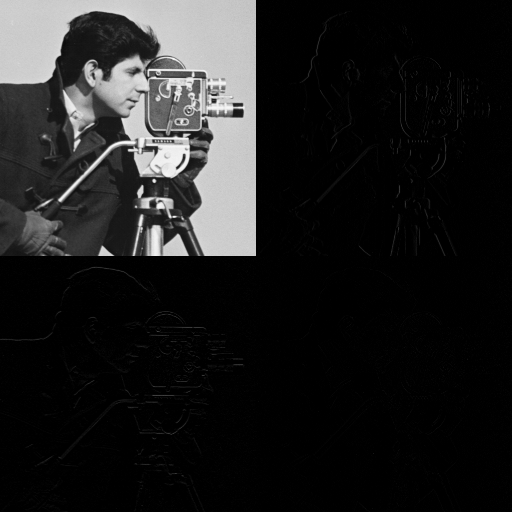
\includegraphics[width=75mm]{../../2_Software/data/cman_HWT.png}
	\caption{Cman Forward HWT.}
	\label{fig:HWT_cman}	
\end{figure}
 
\subsection{Daubechies Wavelet Transform}
The Daubechies Wavelet Transforms, discovered by mathematician Ingrid Daubechies, are a family of orthogonal bases that are conceptually similar to the HWT in that the mathematical computations are running averages and a differences via scalar products \cite{porwik2004haar}. Being that the HWT and Daubechies Wavelet Transform have similar characteristics the HWT is also referred to as the 'DB1' transform. This project solely implements the 'DB4' wavelet algorithm, which utilizes four wavelet and scaling function coefficients. This Daubechies wavelet type has a balanced frequency response but a non-linear phase response. The coefficients in the DB4 wavelet are as follows in equation \eqref{eqn:DB4_coeff}:

\begin{equation}
	c_{0}=\frac{1+\sqrt{3}}{4\sqrt{2}},
	c_{1}=\frac{3+\sqrt{3}}{4\sqrt{2}},
	c_{2}=\frac{3-\sqrt{3}}{4\sqrt{2}},
	c_{3}=\frac{1-\sqrt{3}}{4\sqrt{2}}
	\label{eqn:DB4_coeff}
\end{equation}

\subsection{Thresholding}
Pixel thresholding is often a simple but efficient non-linear denoising approach in the application of a wavelet transform. The thresholding is performed on the wavelet transformed image, and then the image is inverse wavelet transformed to yield a filtered output image. To determine the best threshold value to set, the $detThreshold$ function from $dataSetup.py$ was used. This function first iterates through thresholding values, then thresholds the Wavelet Transformed image, then inverse Wavelet Transforms the thresholded image, and finally calculates the Peak Signal to Noise ratio of the filtered image. The step size of $0.5*std$ where $std$ is the standard deviation of the Gaussian Noise was chosen to allow for a high enough resolution to see how the Threshold effects the PSNR, where the threshold is chosen based off of the one that results in the largest Peak Signal to Noise Ratio. Figure~\ref{fig:psnr_threshold} depicts this PSNR vs. Threshold graph. The following Equations \eqref{eqn:Hard Threshold} and \eqref{eqn:Soft Threshold} detail the Hard and Soft Thresholding calculations respectively, with Figure~\ref{fig:thresholding} depicting the thresholds.
\\\\
Hard Thresholding   
\begin{equation}\label{eqn:Hard Threshold}
D^H(d|T) =
\begin{cases}
0, & \text{if $|d| \leq T$} \\
d, & \text{if $|d| > T$} \\
\end{cases}
\end{equation}	
Soft Thresholding
\begin{equation}\label{eqn:Soft Threshold}
D^S(d|T) =
\begin{cases}
0, & \text{if $|d| \leq T$} \\
d-T, & \text{if $d > T$} \\
d+T, & \text{if $d < -T$}
\end{cases}
\end{equation} 
\begin{figure}[h!]
	\centering
	\begin{subfigure}[b]{0.4\linewidth}
		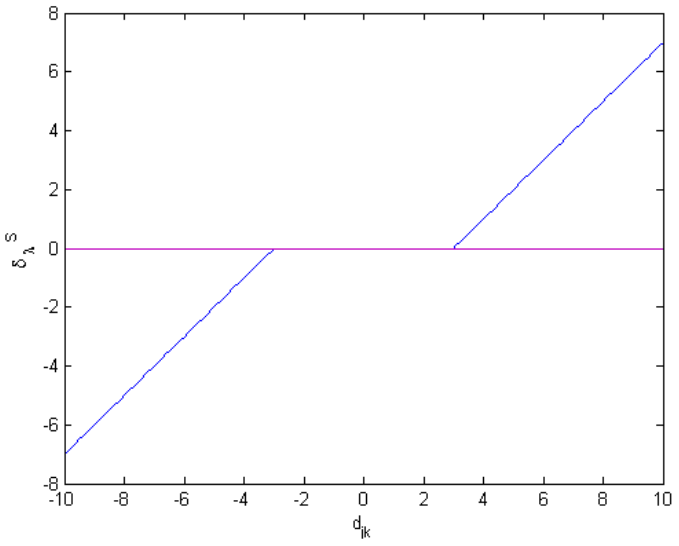
\includegraphics[width=\linewidth]{../../1_Resources/images/hard_thresholding.png}
		\caption{Hard Threshold.}
	\end{subfigure}
	\begin{subfigure}[b]{0.4\linewidth}
		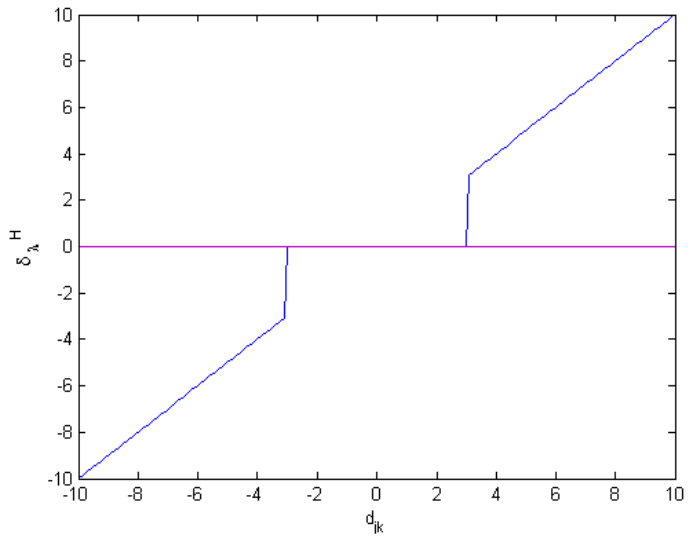
\includegraphics[width=\linewidth]{../../1_Resources/images/soft_thresholding.png}
		\caption{Soft Threshold.}
	\end{subfigure}	
	\caption{Thresholding Methods}
	\label{fig:thresholding}
\end{figure}

The following Figure~\ref{fig:psnr_threshold} depicts the PSNR of the filtered wavelet transforms vs. a given threshold value, and the threshold value was chosen that resulted in the greatest PSNR value.

\begin{figure}[H]
	\centering
	\begin{subfigure}[b]{0.45\linewidth}
		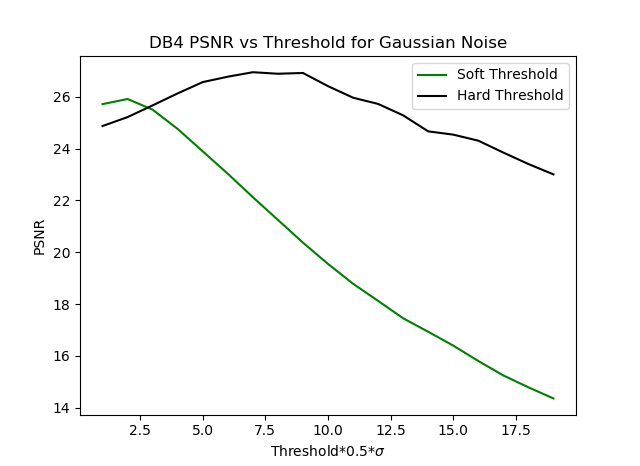
\includegraphics[width=\linewidth]{../../1_Resources/images/DB4_threshold_g.png}
		\caption{DB4 w\ Gaussian Noise}
	\end{subfigure}
	\begin{subfigure}[b]{0.45\linewidth}
		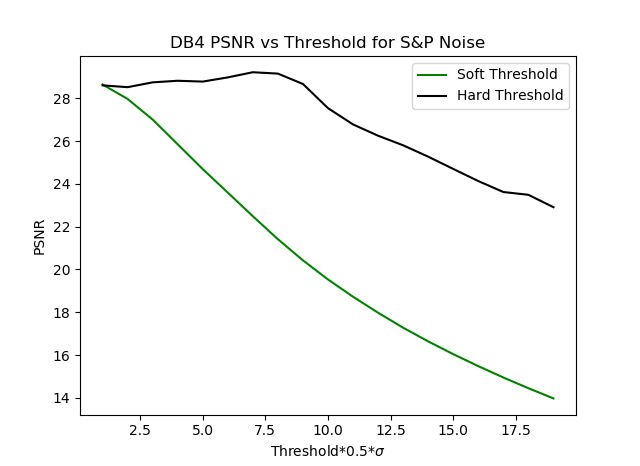
\includegraphics[width=\linewidth]{../../1_Resources/images/DB4_threshold_sp.png}
		\caption{DB4 w\ S\&P Noise}
	\end{subfigure}
	\begin{subfigure}[b]{0.45\linewidth}
		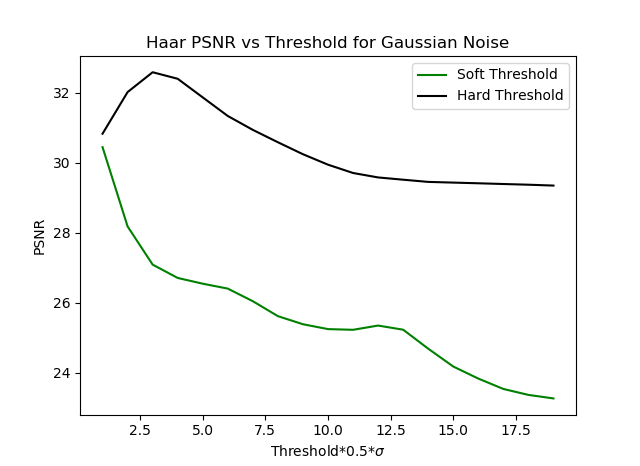
\includegraphics[width=\linewidth]{../../1_Resources/images/HWT_threshold_g.png}
		\caption{HWT w\ Gaussian Noise}
	\end{subfigure}
	\begin{subfigure}[b]{0.45\linewidth}
		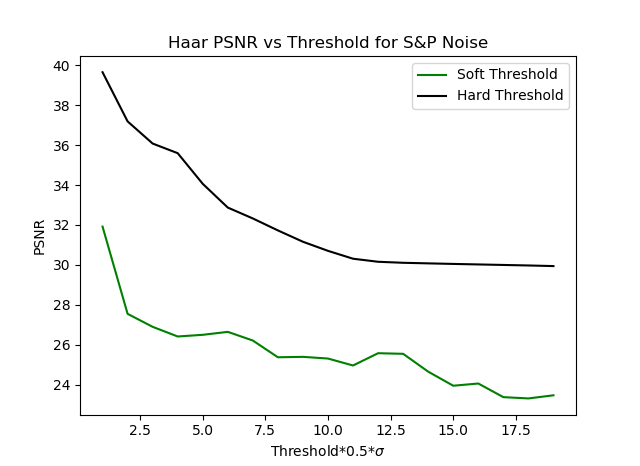
\includegraphics[width=\linewidth]{../../1_Resources/images/HWT_threshold_sp.png}
		\caption{HWT w\ S\&P Noise.}
	\end{subfigure}	
	\caption{PSNR vs. Thresholding Value}
	\label{fig:psnr_threshold}
\end{figure}


\section{Results}\raggedbottom
The following Table \ref{tab:psnr_results} depicts the PSNR results over each filter on their corresponding Gaussian and S\&P noisy images.

\begin{table}[H]
	\centering
	\csvautotabular{../../2_Software/psnr_final.csv}
	\caption{PSNR Filter Results}
	\label{tab:psnr_results}
\end{table}

\subsection{Gaussian Noise Results} 
From observing the PSNR w/ Gaussian Noise we can see that the Bilateral filter appears to yield the highest PSNR with it implementing a filter of length 5. At first this appears strange due to Bilaterally Filtered image in Figure~\ref{fig:filter_outputs_1} not appearing to have the most aesthetically pleasing look to it, however, when reviewed, the PSNR simply returns the "Peak" signal to noise ratio compared to that of the original non-noisy image, and this is not a strong indicator of human aesthetics. This being said, the effects of all of the filters, aside from the DB4 filters, on the Gaussian noise produce a similar PSNR, and this is due to the fact that the Gaussian noise corrupts the original signals PSNR large enough that in order for a filter to yield a greater PSNR it must have a filter length greater than 1 in order to smooth out some of the Gaussian noise. In the case of the Soft and Hard HWT Thresholded images the hard threshold visually and numerically retains the edges in the image, and thus, yields a higher PSNR. The noise in the DB4 transformed images seems to visually appear slightly more reduced than in the HWT images, but the PSNR is significantly lower. This is due to the fact that in the DB4 transform the coefficients, seen previously in equation \eqref{eqn:DB4_coeff}, are scaled significantly larger and significantly smaller than in the HWT and therefore it numerically effects the images pixel values in a greater capacity which results in a higher pixel error in the calculation of the MSE for the PSNR.

\subsection{S\&P Noise Results}
The PSNR results from the S\&P Noise appears to validate the claims made in the previous section on the Gaussian Noise results which is that the intrinsic PSNR of the noisy images vastly differ from the Gaussian noisy image to that of the S\&P noisy image. The S\&P PSNR values from Table \ref{tab:psnr_results} illustrate that the original PSNR of the image is the maximum PSNR without any additional filtering methods. The filter lengths implemented in the $Blur$, $Gaussian$ $Blur$, and $Median$ filters are of length 1, which computationally wise does nothing to the output image. It is not until the S\&P percentage or the original S\&P noisy image becomes larger, upwards of $10\%$, that the filter lengths begin to change for the standard filters in order to lower the PSNR value. The HWT results in a higher PSNR because it is essentially applying a smoothing filter to pairwise pixel values and therefore reducing some S\&P noise, however, it is also pairwise differentiating values which results in a difference in the signal power from the original image. Finally, the DB4 filter appears to have little to no effect on the visuals of the image, and it significantly decreases the outputted PSNR value. The reason for this decrease in value is similar to that in the Gaussian Noise case in that since the original S\&P noisy image has such few corrupted pixels that inducing a scaling coefficient from the DB4 filter and then thresholding the image will result and a higher deviated output image than the original. 

\begin{figure}[H]
	\centering
	\begin{subfigure}[b]{0.45\linewidth}
		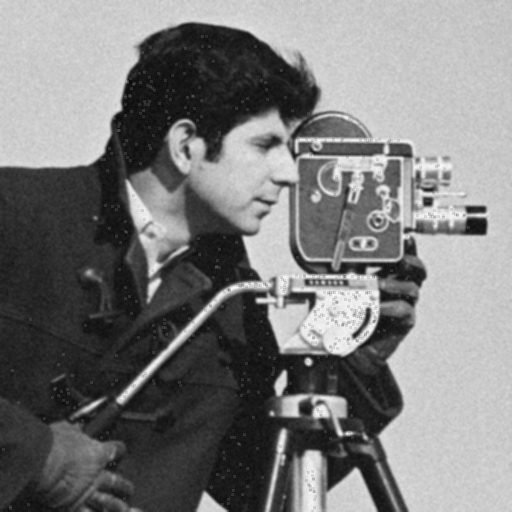
\includegraphics[width=\linewidth]{../../2_Software/data/blur_g.png}
		\caption{Blur}
	\end{subfigure}
	\begin{subfigure}[b]{0.45\linewidth}
		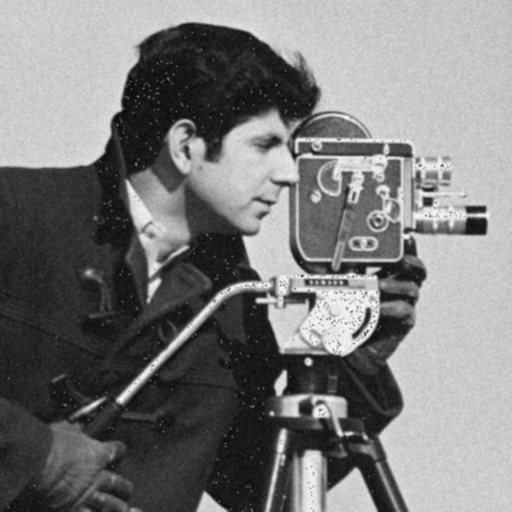
\includegraphics[width=\linewidth]{../../2_Software/data/gblur_g.png}
		\caption{Gaussian Blur}
	\end{subfigure}
	\begin{subfigure}[b]{0.45\linewidth}
		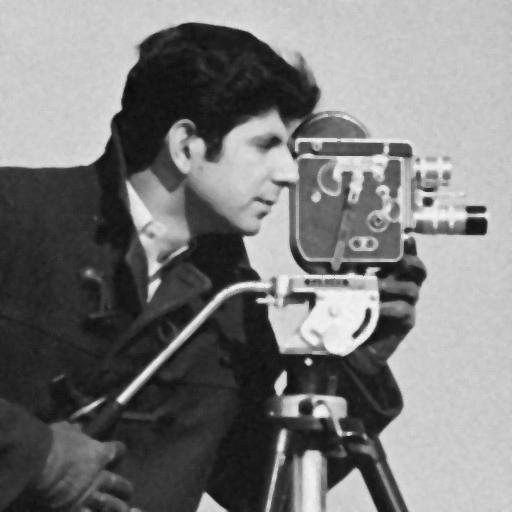
\includegraphics[width=\linewidth]{../../2_Software/data/median_g.png}
		\caption{Median Filter}
	\end{subfigure}
	\begin{subfigure}[b]{0.45\linewidth}
		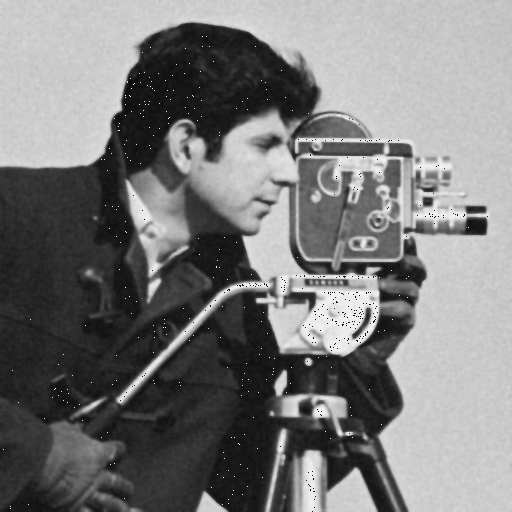
\includegraphics[width=\linewidth]{../../2_Software/data/bilateral_g.png}
		\caption{Bilateral Filter}
	\end{subfigure}
	\begin{subfigure}[b]{0.45\linewidth}
		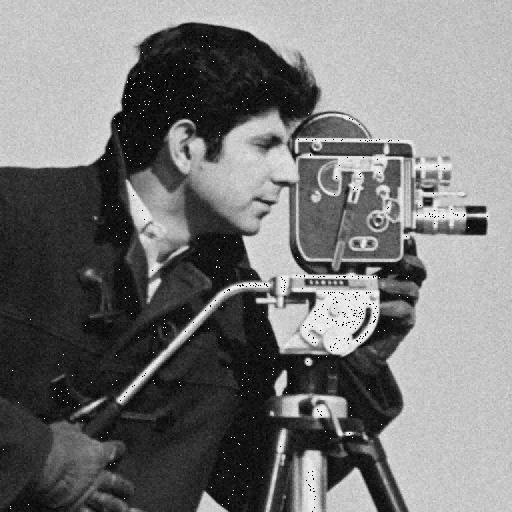
\includegraphics[width=\linewidth]{../../2_Software/data/IHWT_soft_g.png}
		\caption{Soft Threshold HWT}
	\end{subfigure}
	\begin{subfigure}[b]{0.45\linewidth}
		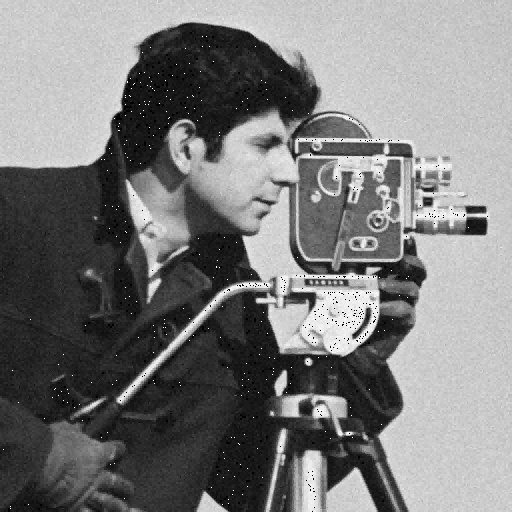
\includegraphics[width=\linewidth]{../../2_Software/data/IHWT_hard_g.png}
		\caption{Hard Threshold HWT}
	\end{subfigure}	
	\caption{Filter Outputs on Gaussian Noise}	
	\label{fig:filter_outputs_1}
\end{figure}

\begin{figure}[H]
	\centering
	\begin{subfigure}[b]{0.45\linewidth}
		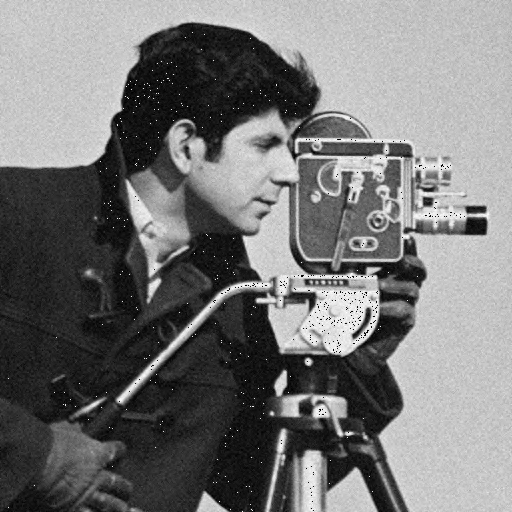
\includegraphics[width=\linewidth]{../../2_Software/data/IDB4T_soft_g.png}
		\caption{Soft Threshold DB4T}
	\end{subfigure}
	\begin{subfigure}[b]{0.45\linewidth}
		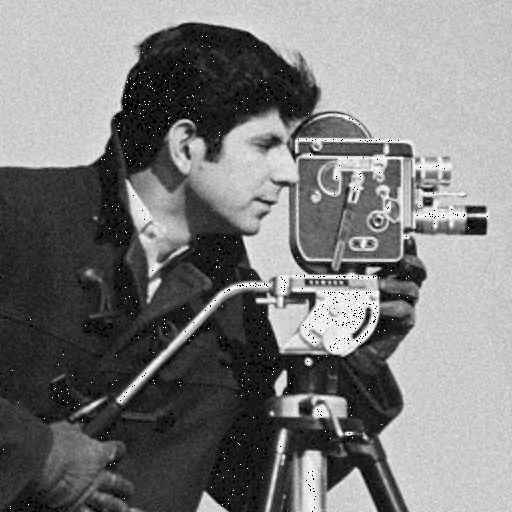
\includegraphics[width=\linewidth]{../../2_Software/data/IDB4T_hard_g.png}
		\caption{Hard Threshold DB4T}
	\end{subfigure}
	\caption{Filter Outputs on Gaussian Noise cont.}
	\label{fig:filter_outputs_2}
\end{figure}

\begin{figure}[H]
	\centering
	\begin{subfigure}[b]{0.45\linewidth}
		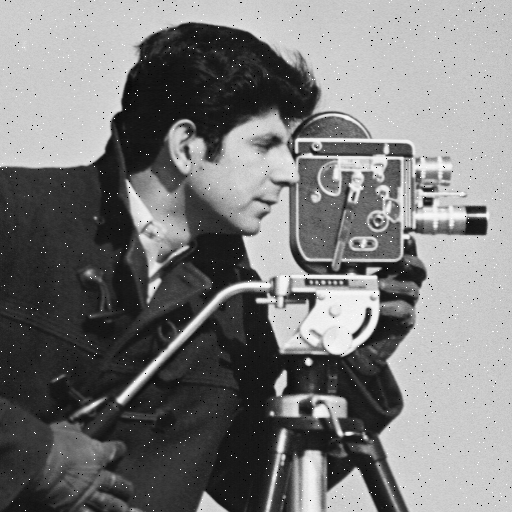
\includegraphics[width=\linewidth]{../../2_Software/data/blur_sp.png}
		\caption{Blur}
	\end{subfigure}
	\begin{subfigure}[b]{0.45\linewidth}
		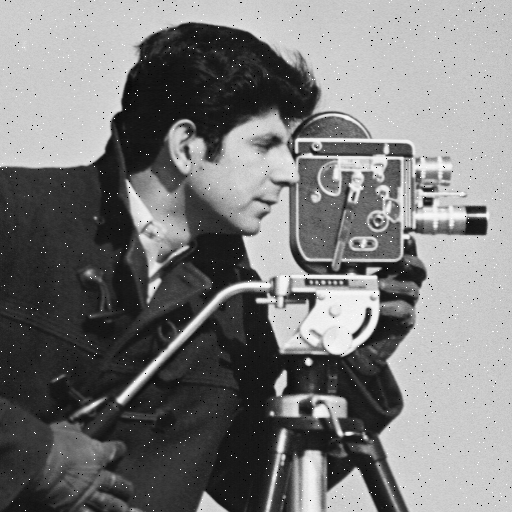
\includegraphics[width=\linewidth]{../../2_Software/data/gblur_sp.png}
		\caption{Gaussian Blur}
	\end{subfigure}

	\caption{Filter Outputs on S\&P Noise}
	\label{fig:filter_outputs_3}
\end{figure}

\begin{figure}[H]
	\centering
		\begin{subfigure}[b]{0.45\linewidth}
		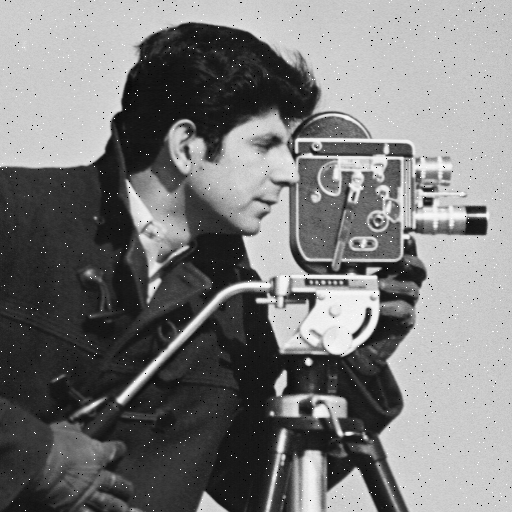
\includegraphics[width=\linewidth]{../../2_Software/data/median_sp.png}
		\caption{Median Filter}
	\end{subfigure}
	\begin{subfigure}[b]{0.45\linewidth}
		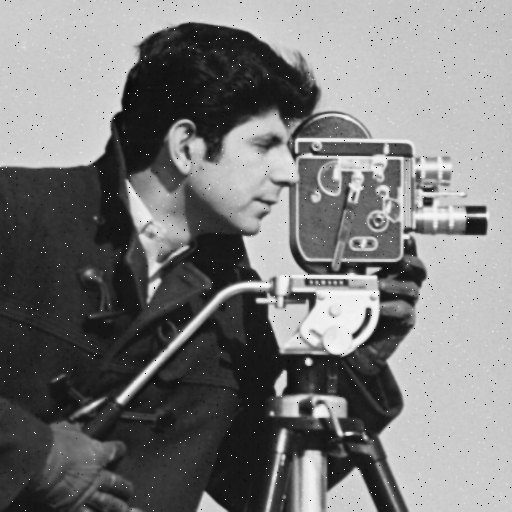
\includegraphics[width=\linewidth]{../../2_Software/data/bilateral_sp.png}
		\caption{Bilateral Filter}
	\end{subfigure}
	\begin{subfigure}[b]{0.45\linewidth}
		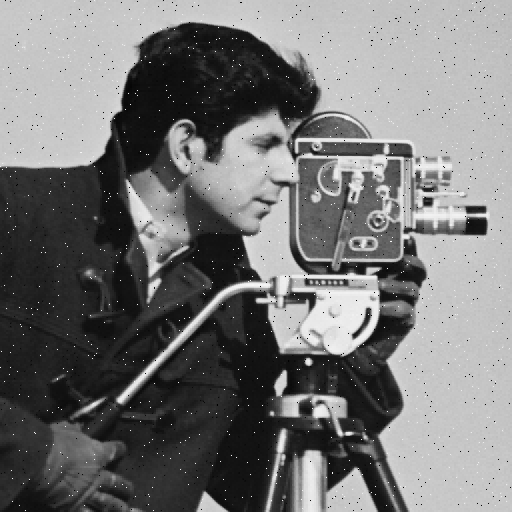
\includegraphics[width=\linewidth]{../../2_Software/data/IHWT_soft_sp.png}
		\caption{Soft Threshold HWT}
	\end{subfigure}
	\begin{subfigure}[b]{0.45\linewidth}
		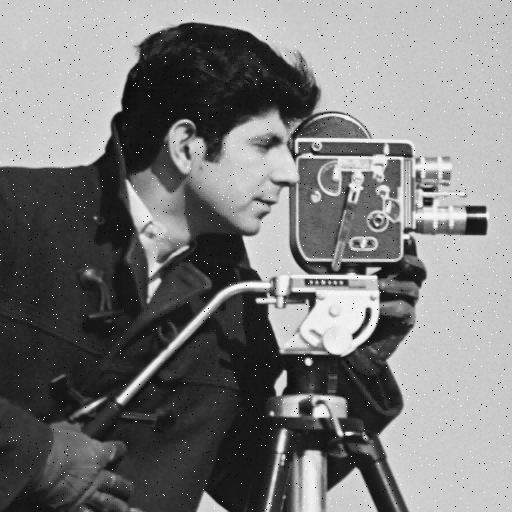
\includegraphics[width=\linewidth]{../../2_Software/data/IHWT_hard_sp.png}
		\caption{Hard Threshold HWT}
	\end{subfigure}
	\begin{subfigure}[b]{0.45\linewidth}
		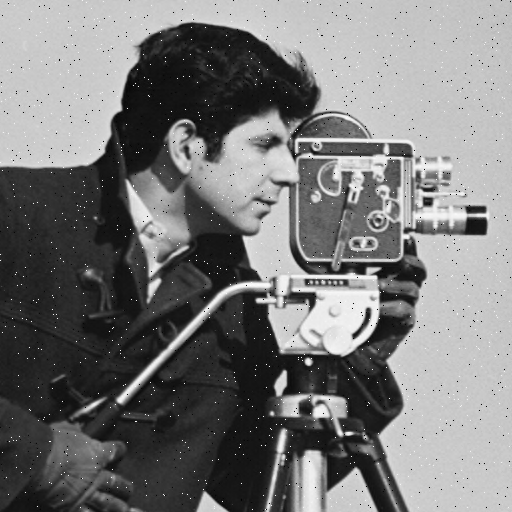
\includegraphics[width=\linewidth]{../../2_Software/data/IDB4T_soft_sp.png}
		\caption{Soft Threshold DB4T}
	\end{subfigure}
	\begin{subfigure}[b]{0.45\linewidth}
		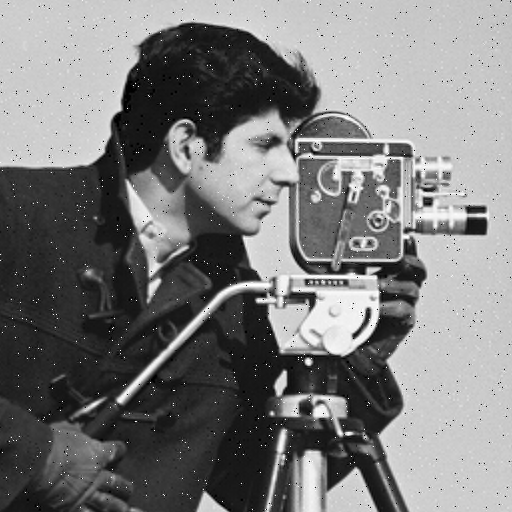
\includegraphics[width=\linewidth]{../../2_Software/data/IDB4T_hard_sp.png}
		\caption{Hard Threshold DB4T}
	\end{subfigure}
	\caption{Filter Outputs on S\&P Noise cont.}
	\label{fig:filter_outputs_4}
\end{figure}


\section{Conclusion}
In the present work, multiple filters are evaluated from observations of their corresponding filtered output image's PSNR values. The standard library $Blur$, $Gaussian$ $Blur$, $Median$, and $Bilateral$ filters have been specifically tuned in filter length size in order to produce the highest outputted PSNR value. Along with these filters, the HWT and the DB4 filters have been tuned via a thresholding parameter in order to yield a larger PSNR output. From this paper one can conclude that the PSNR value has little impact on the visual "goodness" of an image, but rather, it is a method of comparing two similar images and the noise distribution. In review of this project a more in depth analysis on different wavelet techniques would be beneficial to see how changing wavelet taps/coefficients effects outputted images. Also, a different method other than the PSNR to compare the outputted image to the original would be desired. Potentially looking at the Structural Similarity Index of the images, which is a method of measuring image quality similarity between two images could provide more insight into a more appropriate approach of evaluation.

\section{References}


\bibliography{bibfile} 
\bibliographystyle{unsrt}

\clearpage
\section{Software Lisiting}\label{Software_Lisiting}
\subsection{dataSetup}
\lstinputlisting[language=Python]{../../2_Software/dataSetup.py}
\clearpage
\subsection{DWT}
\lstinputlisting[language=Python]{../../2_Software/DWT.py}
\end{document}